\documentclass[11pt,a4paper]{article}
\usepackage[margin=2cm]{geometry}
\usepackage{amsmath,amssymb,mathtools}
\usepackage{booktabs,longtable,float,graphicx,enumitem}
\usepackage[table]{xcolor}
\usepackage{tikz}
\usetikzlibrary{arrows.meta,positioning}
\usepackage{listings}
\usepackage{microtype}
\usepackage[hidelinks]{hyperref}
\lstset{basicstyle=\ttfamily\scriptsize,breaklines=true,columns=fullflexible,frame=single,keepspaces=true}
\setlength{\parindent}{0pt}
\setlength{\parskip}{4pt}

% ---- edit before submitting -------------------------------------------------
\newcommand{\studentname}{Erik Mirzoyan}  % fill in
\newcommand{\studentid}{\rule{3.5cm}{0.4pt}}     % fill in
\newcommand{\repourl}{https://github.com/10mirzoyan71/photonicsai-hw2}
\newcommand{\videonote}{\texttt{hw2\_agentic\_hardware/video/task2\_agent\_run.mp4} in the repository (the run reported below)}
% -----------------------------------------------------------------------------
\newcommand{\todobox}[1]{\begin{center}\fcolorbox{red}{red!5}{\begin{minipage}{0.92\linewidth}#1\end{minipage}}\end{center}}

% generated by hw2_agentic_hardware/validate_bench.py
\newcommand{\specklecontrast}{0.98}
\newcommand{\specklegrain}{2.5}
\newcommand{\shotnoise}{7.1}
\newcommand{\validationtable}{\begin{tabular}{@{}rrrrrrrrr@{}}\toprule macropixel & $N$ & $N_\text{eff}$ & iterations & flips & $\eta$ & $\eta_\text{far}$ & known-$T$ & $N_\text{eff}/2\pi$\\\midrule
16 & 16 & 9 & 400 & 2$\to$1 & 4.3 & 4.4 & 4.1 & 1.4\\
8 & 64 & 32 & 1500 & 4$\to$1 & 9.5 & 9.7 & 8.3 & 5.0\\
4 & 256 & 123 & 6000 & 8$\to$1 & 28.5 & 30.7 & 28.7 & 19.6\\
2 & 1024 & 491 & 20000 & 16$\to$1 & 96.6 & 61.3 & 95.1 & 78.1\\
1 & 4096 & 1960 & 20000 & 32$\to$1 & 287.4 & 107.2 & 373.1 & 312.0\\
\bottomrule\end{tabular}}
\newcommand{\ringtable}{\begin{tabular}{@{}rcrr@{}}\toprule focus [px] & ring $r$ [px] & $\eta$ (proximal) & $\eta_\text{far}$\\\midrule
$3\times3$ & 6--14 & 41.0 & 18.6\\
$3\times3$ & 4--30 & 28.6 & 26.1\\
$1\times1$ & 4--30 & 38.2 & 40.8\\
$5\times5$ & 4--30 & 15.3 & 13.3\\
\bottomrule\end{tabular}}


\begin{document}
\begin{center}
{\Large\bfseries PhotonicsAI --- AI-Driven Science and Autonomous Laboratories}\\[3pt]
{\large Homework 2: Agentic Systems with Hardware}\\[6pt]
Name: \studentname \qquad Due 12.10.2026\\[2pt]
Code: \url{\repourl}, folder \texttt{hw2\_agentic\_hardware/} (the Homework 1 repository, with this work added)
\end{center}

%======================================================================
\section*{Task 1. Human-in-the-loop}
%======================================================================
\textbf{Code:} \texttt{hw2\_agentic\_hardware/agent\_v2.py} (graph), \texttt{run\_task1.py} (runs a thread, pauses for the
person), \texttt{render\_hw2.py}, \texttt{tests/offline\_tests.py}. It starts from Homework 1, Task 6: the same four roles,
the same shared dialogue as the state of a LangGraph \texttt{StateGraph}, the same role prompts, the same coding tool given
only to the executor, the same 8-decision budget, and the orchestrator's choice is still a model call with structured output.
All runs in this report used \texttt{--model claude-cli:claude-sonnet-5-5}: the model is called through the Claude Code CLI
in print mode (\texttt{task6\_agentic\_system/claude\_cli.py}) with the CLI's own tools switched off; decisions are its
structured output, and the executor's tools (coding, focusing) are requested as structured output and run by the executor node.

\begin{center}
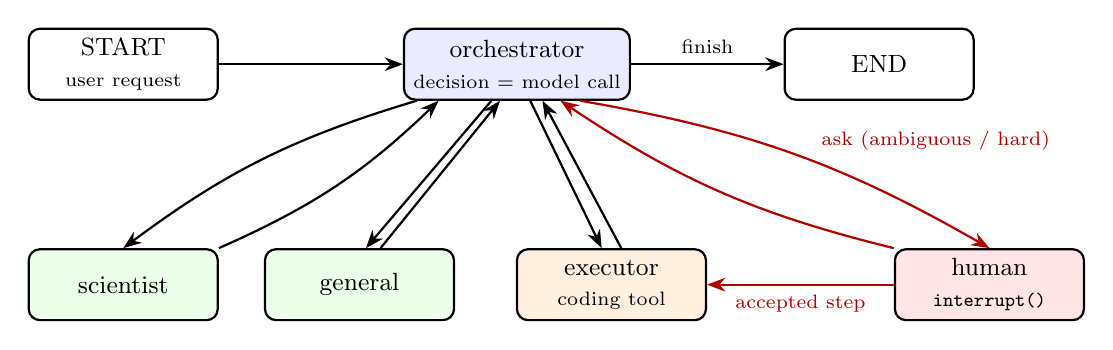
\begin{tikzpicture}[>=Stealth,
  box/.style={draw,thick,rounded corners,minimum width=24mm,minimum height=9mm,align=center,font=\small}]
  \node[box,fill=blue!8] (o) at (0,0) {orchestrator\\\scriptsize decision = model call};
  \node[box] (s) at (-5,0) {START\\\scriptsize user request};
  \node[box] (e) at (4.6,0) {END};
  \node[box,fill=green!8] (sc) at (-5,-2.8) {scientist};
  \node[box,fill=green!8] (g) at (-2,-2.8) {general};
  \node[box,fill=orange!12] (ex) at (1.2,-2.8) {executor\\\scriptsize coding tool};
  \node[box,fill=red!10] (h) at (6.0,-2.8) {human\\\scriptsize \texttt{interrupt()}};
  \draw[->,thick] (s) -- (o);
  \draw[->,thick] (o) -- node[above,font=\scriptsize]{finish} (e);
  \draw[->,thick] (o.200) to[bend right=10] (sc.north);  \draw[->,thick] (sc.north east) to[bend right=10] (o.205);
  \draw[->,thick] (o.235) -- (g.80);  \draw[->,thick] (g.60) -- (o.245);
  \draw[->,thick] (o.290) -- (ex.105);  \draw[->,thick] (ex.75) -- (o.305);
  \draw[->,thick,red!70!black] (o.330) to[bend left=10] node[above right,font=\scriptsize,pos=0.55]{ask (ambiguous / hard)} (h.north);
  \draw[->,thick,red!70!black] (h.north west) to[bend left=10] (o.320);
  \draw[->,thick,red!70!black] (h.west) -- node[below,font=\scriptsize]{accepted step} (ex.east);
\end{tikzpicture}\\[2pt]
{\small Red: the orchestrator asks the person; the reply goes back to the orchestrator (ambiguous query, or refused step) or runs the accepted step.}
\end{center}

\paragraph{When the graph stops.} The orchestrator's structured output is now
\texttt{Decision(next\_role, instruction, question, reason, stop\_kind, pending\_role, pending\_instruction)} with
\texttt{next\_role} $\in\{$scientist, general, executor, \textbf{human}, finish$\}$. Its prompt defines the two situations
and nothing else decides them: an \emph{ambiguous query} (the latest request has more than one reading, and the readings would
send the work to different roles or change the reported number; the question lists the readings), and a \emph{hard decision}
(the next step would run the coding tool, overwrite a result already on disk, or end the dialogue and report a measurement;
the step goes into \texttt{pending\_role}/\texttt{pending\_instruction} and the question states it). To judge overwrites, the
status line the orchestrator reads lists the files already in the working directory. There is no keyword list and no rule
that stops on a fixed role: whether to stop is decided by the model from the dialogue.

\paragraph{How the stop works.} The graph is compiled with a checkpointer, \texttt{SqliteSaver}, whose file is
\texttt{runs/checkpoints.sqlite}, and every run is a thread: \texttt{config = \{"configurable": \{"thread\_id": <id>\}\}}.
The \texttt{human} node calls \texttt{langgraph.types.interrupt(payload)} with the question (and the proposed step); the run
returns with the pending interrupt and the thread stays paused at that node. \texttt{run\_task1.py} prints the question and
reads the reply; \texttt{graph.invoke(Command(resume=reply), config)} resumes the same thread (also from a new process:
\texttt{--thread <id> --reply "..."}). The reply is appended as a turn with role \texttt{human}; then
\begin{itemize}[leftmargin=*,itemsep=1pt]
\item ambiguous: the turn goes back to the orchestrator, whose next decision reads the reply and follows that reading;
\item hard decision, accepted (the reply starts with an explicit yes / ok / proceed / accept): the human node routes straight to
the executor with the pending instruction, or, for a pending finish, the orchestrator writes the approved final report and the
graph ends;
\item hard decision, refused (anything else): the turn goes back to the orchestrator and the step does not run. The orchestrator's
next turn starts with a record computed in code, ``the proposed step (\dots) was REFUSED by the human and did NOT run. Tool calls
in this run: $n$ when it was proposed, $n$ now.''
\end{itemize}
The Homework 1 rule stays: finishing (directly or as a pending step) needs an executor turn with a VERIFIED measurement.

\subsection*{Run (a): an ambiguous request about the Silverbox work}
Thread \texttt{run\_a}. \textbf{Request typed to the orchestrator:} \emph{What is the error of our Silverbox model?}
\textbf{Stop 1 (turn 2, ambiguous): the question the graph posed:}
\begin{lstlisting}
Decision 1/8 -> human (ambiguous)
Question: Which error do you mean? (a) Free-run RMSE of the kept PINN (A2_h5), on test data, train data, or both; (b) the same for the 4-coefficient Duffing reference (R_duffing), or a PINN vs Duffing comparison; (c) something else, such as one-step-ahead error or the full 26-run table from summary.md?
Reason: "Error of our Silverbox model" has several readings that would report different numbers.
\end{lstlisting}

\textbf{Reply typed (turn 3, role \texttt{human}):}
\begin{lstlisting}
the free-run test RMSE of the kept PINN network, recomputed from the saved weights
\end{lstlisting}

\textbf{Next message in the dialogue (turn 4, orchestrator):}
\begin{lstlisting}
Decision 2/8 -> human (hard decision)
Proposed step: executor: In silverbox/silverbox_pinn.py, use load_excerpt (data/SNLS80mV.mat), load_model (silverbox/results/A2_h5.pt, with the config in A2_h5.json) and free_run to recompute the free-run RMSE of the kept PINN A2_h5 on the TEST segment, using the saved weights. Don't train. Don't write or overwrite any files on disk. Print the test RMSE, and also the value stored in A2_h5.json (and kept.json) for comparison. Report exactly what the tools return, and report any traceback.
Question: To recompute the free-run test RMSE of the kept PINN (A2_h5), I need to run code. Shall I proceed? It will load the weights from silverbox/results/A2_h5.pt with load_model, load the test excerpt from data/SNLS80mV.mat with load_excerpt, and run free_run. It will then report the test RMSE and compare it with the value stored in A2_h5.json. It won't write or overwrite any files.
Reason: Running the coding tool is a hard decision, so I need approval before the executor recomputes the RMSE.
\end{lstlisting}

The run continued with 2 more stop(s) until the end (turn 13); all turns are in the table.
\textbf{All turns of this run:}
\begin{longtable}{@{}r l p{0.74\linewidth}@{}}
\toprule \# & role & what it did\\ \midrule \endhead
1 & user & What is the error of our Silverbox model? (Context: the working directory holds my Homework 1 Silverbox work: the record data/SNLS80mV.mat, the code silverbox/silverbo...\\
2 & orchestrator & -\textgreater{} human (ambiguous): "Error of our Silverbox model" has several readings that would report different numbers.\\
3 & human & reply: the free-run test RMSE of the kept PINN network, recomputed from the saved weights\\
4 & orchestrator & -\textgreater{} human (hard\_decision): Running the coding tool is a hard decision, so I need approval before the executor recomputes the RMSE.\\
5 & human & reply: yes, proceed [accepted]\\
6 & executor & write inspect\_sb.py: ok run inspect\_sb.py: exit code 0, 0.1 s write inspect\_sb2.py: write budget for this turn is used; run the file and report run inspect\_sb2.py: ins...\\
7 & orchestrator & -\textgreater{} executor: The user already approved the recompute run, and the executor still needs the function signatures before it can compute the RMSE.\\
8 & executor & write inspect\_sb3.py: ok run inspect\_sb3.py: exit code 0, 1.5 s\\
9 & orchestrator & -\textgreater{} executor: The user already approved this exact recompute run, and the executor now has the function signatures it needs.\\
10 & executor & write recompute\_a2h5.py: ok run recompute\_a2h5.py: exit code 0, 2.2 s VERIFIED printed by the script: \{'test': 0.00042225465297085084, 'train': 0.00040721431617798747\}\\
11 & orchestrator & -\textgreater{} human (hard\_decision): Finishing and reporting a measurement is a hard decision, so I need approval first.\\
12 & human & reply: yes, finish and report [accepted]\\
13 & orchestrator & Final report (accepted by the human): The free-run test RMSE of the kept PINN network (A2\_h5), recomputed from the saved weights A2\_h5.pt with load\_excerpt, load\_model...\\
\bottomrule
\end{longtable}

\subsection*{Run (b): a hard decision, refused once, then accepted}
Thread \texttt{run\_b}. \textbf{Request typed to the orchestrator:} \emph{Re-evaluate the kept Silverbox network and update silverbox/results/kept.json with the new numbers.}
\textbf{Stop 1 (turn 4, hard decision): the question the graph posed:}
\begin{lstlisting}
Decision 2/8 -> human (hard decision)
Proposed step: executor: Execute the scientist's plan. 1) Read and print silverbox/results/kept.json in full and keep a copy as old. 2) Read and print silverbox/results/A2_h5.json, and read the source of load_excerpt, load_model, free_run and half_sample_input in silverbox/silverbox_pinn.py. 3) Using the excerpt and settings recorded in A2_h5.json, load the data and the A2_h5.pt network and run free_run on the train and test segments. Run from the project root with a 5-minute wall-clock guard. Check that the values are finite. Print TRAIN_RMSE=<float> and TEST_RMSE=<float>. 4) If kept.json holds an R_duffing entry, run the same evaluation for R_duffing.pt and R_duffing.json. Otherwise skip it and do not add one. 5) Print the old and new train and test RMSE side by side, with absolute and relative differences. Flag differences above 1%. Also compare with the A2_h5.json and summary.md values. 6) Save a backup of kept.json as kept.json.bak. Then overwrite silverbox/results/kept.json, changing only the RMSE fields (and a date field, if one exists) and keeping the same keys, key order and indent. Reload the file and verify that the keys match old and that only the intended values changed. 7) Report the old and new numbers, the fields changed, and 
[... abridged ...]
verbox/results/kept.json with the new RMSE values, keeping the existing schema. It will save a backup, kept.json.bak, before writing. Shall I proceed?
Reason: The executor step runs code and overwrites the existing silverbox/results/kept.json, so the person must approve it first.
\end{lstlisting}

\textbf{Reply typed (turn 5, role \texttt{human}):} \textbf{refused}.
\begin{lstlisting}
no, do not overwrite kept.json
\end{lstlisting}

\textbf{Next message in the dialogue (turn 6, orchestrator):}
\begin{lstlisting}
Record: the proposed step (executor: Execute the scientist's plan. 1) Read and print silverbox/results/kept.json in full and keep a copy as old. 2) Read and print silverbox/results/A2_h5.json, and read the source of load_excerpt, load_model, free_run and half_sample_input in silverbox/silverbox_pinn.py. 3) Using the excerpt and setting) was REFUSED by the human and did NOT run. Tool calls in this run: 0 when it was proposed, 0 now.
Decision 3/8 -> human (hard decision)
Proposed step: executor: READ-ONLY re-evaluation. Do NOT write, overwrite or modify any file, in particular silverbox/results/kept.json, and do not create backups or plots in the project. 1) Read and print silverbox/results/kept.json in full and keep a copy as old. 2) Read and print silverbox/results/A2_h5.json, and read the source of load_excerpt, load_model, free_run and half_sample_input in silverbox/silverbox_pinn.py. 3) Using the excerpt and settings recorded in A2_h5.json, load the data and the A2_h5.pt network. Run free_run on the train and test segments from the project root with a 5-minute wall-clock guard. Check that the values are finite. Print TRAIN_RMSE=<float> and TEST_RMSE=<float>. 4) If kept.json holds an R_duffing entry, run the same evaluation for R_duffing.pt and R_duffing.json. Otherwise skip it
[... abridged ...]
 new numbers side by side. It would not write or modify any file on disk, including kept.json, and it would not create a backup. Proceed with this read-only run?
Reason: The overwrite was refused, so I'm proposing a read-only re-evaluation. Any executor turn still needs approval.
\end{lstlisting}

\textbf{Stop 2 (turn 6, hard decision): the question the graph posed} is the message above (turn 6).
\textbf{Reply typed (turn 7, role \texttt{human}):} accepted.
\begin{lstlisting}
yes, proceed with the read-only re-evaluation
\end{lstlisting}

\textbf{Next message in the dialogue (turn 8, executor):}
\begin{lstlisting}
The re-evaluation did not run, so I have no new RMSE numbers to report.

- What ran: ro_inspect.py exited with code 0. It only printed kept.json, A2_h5.json, R_duffing.json, summary.md and silverbox_pinn.py. The returned stdout was truncated at the start, so I only saw the tail of silverbox_pinn.py (the end of train and load_model). I did not see kept.json, the A2_h5.json settings or summary.md, so I have no old RMSE values to compare.
- What failed: I tried to write a second script, ro_inspect2.py, to print the files without the history and show the source of load_excerpt, free_run and half_sample_input. The tool refused with "write budget for this turn is used". The run call then failed because the file doesn't exist.
- Not done: I did not call load_excerpt, load_model or free_run. I printed no TRAIN_RMSE= or TEST_RMSE=, did no R_duffing check, and made no comparison against A2_h5.json or summary.md.
- Files: silverbox/results/kept.json is unchanged. I didn't write a backup or a plot. The only file I created is ro_inspect.py in the working directory, which is read-only in behavior.

I need one more turn with a write allowed to finish. The script would print kept.json and the A2_h5.json settings (without the history), read the function sources, and run the evaluation. Do you want me to continue?

[tool record]
write ro_inspect.py: ok
run ro_inspect.py: exit code 0, 0.1 s
write ro_inspect2.py: write budget for this turn is used; run the file and report
run ro_inspect2.py: ro_inspect2.py does not exist in the working directory
\end{lstlisting}

The run continued with 1 more stop(s) until the end (turn 15); all turns are in the table.
\textbf{All turns of this run:}
\begin{longtable}{@{}r l p{0.74\linewidth}@{}}
\toprule \# & role & what it did\\ \midrule \endhead
1 & user & Re-evaluate the kept Silverbox network and update silverbox/results/kept.json with the new numbers. (Context: the working directory holds my Homework 1 Silverbox work:...\\
2 & orchestrator & -\textgreater{} scientist: No plan exists yet; the scientist must specify how to re-evaluate the kept network A2\_h5 (free-run train/test RMSE using the silverbox\_pinn.py functions)...\\
3 & scientist & \# Plan: re-evaluate the kept Silverbox PINN (A2\_h5) and update kept.json **Model and test (unchanged from Homework 1).** The Silverbox is a Duffing-type oscillator, y'...\\
4 & orchestrator & -\textgreater{} human (hard\_decision): The executor step runs code and overwrites the existing silverbox/results/kept.json, so the person must approve it first.\\
5 & human & reply: no, do not overwrite kept.json [refused]\\
6 & orchestrator & [refused step recorded as not run] -\textgreater{} human (hard\_decision): The overwrite was refused, so I'm proposing a read-only re-evaluation. Any executor turn still needs appro...\\
7 & human & reply: yes, proceed with the read-only re-evaluation [accepted]\\
8 & executor & write ro\_inspect.py: ok run ro\_inspect.py: exit code 0, 0.1 s write ro\_inspect2.py: write budget for this turn is used; run the file and report run ro\_inspect2.py: ro\_...\\
9 & orchestrator & -\textgreater{} executor: The person already approved the read-only re-evaluation, and the executor only needs to finish it. It needs one script that does everything in a single wr...\\
10 & executor & write ro\_inspect.py: ro\_inspect.py already exists; every implementation goes into a NEW file (e.g. a new version suffix) run ro\_inspect.py: exit code 0, 0.0 s write ro...\\
11 & orchestrator & -\textgreater{} executor: The person already approved the read-only re-evaluation, and ro\_inspect3.py is written, so the executor only needs to run it.\\
12 & executor & run ro\_inspect3.py: exit code 0, 2.7 s VERIFIED printed by the script: \{'test': 0.000422255, 'train': 0.000407214\}\\
13 & orchestrator & -\textgreater{} human (hard\_decision): Finishing and reporting a measurement is a hard decision, so I need approval before ending the run.\\
14 & human & reply: yes, finish and report [accepted]\\
15 & orchestrator & Final report (accepted by the human): Read-only re-evaluation of the kept Silverbox network A2\_h5 (free run, excerpt of 4096 samples, train/test split at sample 3072, ...\\
\bottomrule
\end{longtable}


%======================================================================
\section*{Task 2. Focusing through a simulated bench}
%======================================================================
\textbf{Code:} \texttt{hw2\_agentic\_hardware/bench.py} (bench, search, tool), \texttt{agent\_v2.py} (the executor receives the
tool), \texttt{run\_task2.py}, \texttt{validate\_bench.py}. Screen recording: \videonote.

\subsection*{The simulated bench}
The imaging part of the path, laser $\to$ DMD $\to$ scattering medium $\to$ camera, is
\[
I_\text{cam}=\mathcal N\!\left(\kappa\,\big|T E_\text{in}\big|^2\right),\qquad (E_\text{in})_j=a_j\,s_j,\quad s_j\in\{0,1\},
\]
\begin{itemize}[leftmargin=*,itemsep=1pt]
\item DMD: $64\times64$ mirrors, binary amplitude $s_j$; the expanded beam illuminates it with a Gaussian amplitude $a_j$ (waist
0.8 of the half side). A macropixel of $m\times m$ mirrors switches together, so $N=(64/m)^2$ segments.
\item $T$ ($4096$ camera pixels $\times$ $4096$ mirrors): each column, the field one mirror makes on the camera, is an independent
fully developed speckle field (circular Gaussian noise low-passed by a circular pupil). Measured on a random pattern: contrast
\specklecontrast, speckle grain \specklegrain\,px (FWHM of the intensity autocorrelation).
\item Camera $\mathcal N$: Poisson shot noise (mean signal 400\,e$^-$/px for a random half-on pattern), 5\,e$^-$ read noise, 1\%
laser intensity noise per shot, full-well clipping. Two shots of the same pattern differ by \shotnoise\% rms per pixel.
\end{itemize}

\subsection*{The search and the tool}
\texttt{focusing\_tool(macropixel, focus\_size, bg\_inner, bg\_outer, bg\_regions, iterations, flips, flips\_final, remeasure,
final\_shots)} follows the algorithm of the task: random start; after every shot the mean intensity in the focus square and in
\texttt{bg\_regions} angular sectors of the ring $r_\text{in}<r\le r_\text{out}$ around it is read;
\[
\eta=\frac{\langle I\rangle_\text{focus}}{\frac1K\sum_{k=1}^{K}\langle I\rangle_{\text{region }k}};
\]
each iteration flips \texttt{flips} random macropixels (annealed to \texttt{flips\_final}) and keeps the flip if $\eta$ rose
(with \texttt{remeasure} the current pattern is re-shot every iteration so a lucky noisy reading cannot lock in). It returns
$\eta$ (mean $\pm$ std over fresh final shots), $\eta_\text{far}$ (the focus against the camera outside the ring, which the search
never sees), the progress trace, and the images (random-start camera, final camera with the regions drawn, DMD pattern, trace).
The executor is the only role that receives it; with it the system runs without the human stop, so after ``focus the beam'' it
chooses every setting itself.

\subsection*{Bench validation (run directly, not by the agent)}
\begin{center}\small\validationtable\end{center}
$\eta$ is the task's metric, $\eta_\text{far}$ the focus against the rest of the camera, ``known-$T$'' the best binary pattern
built from the transmission matrix (segments in phase with the focus, threshold scanned), and $N_\text{eff}/2\pi$ the
binary-amplitude theory for a Gaussian-illuminated DMD ($N_\text{eff}=(\sum A_k^2)^2/\sum A_k^4$).
\begin{figure}[H]\centering
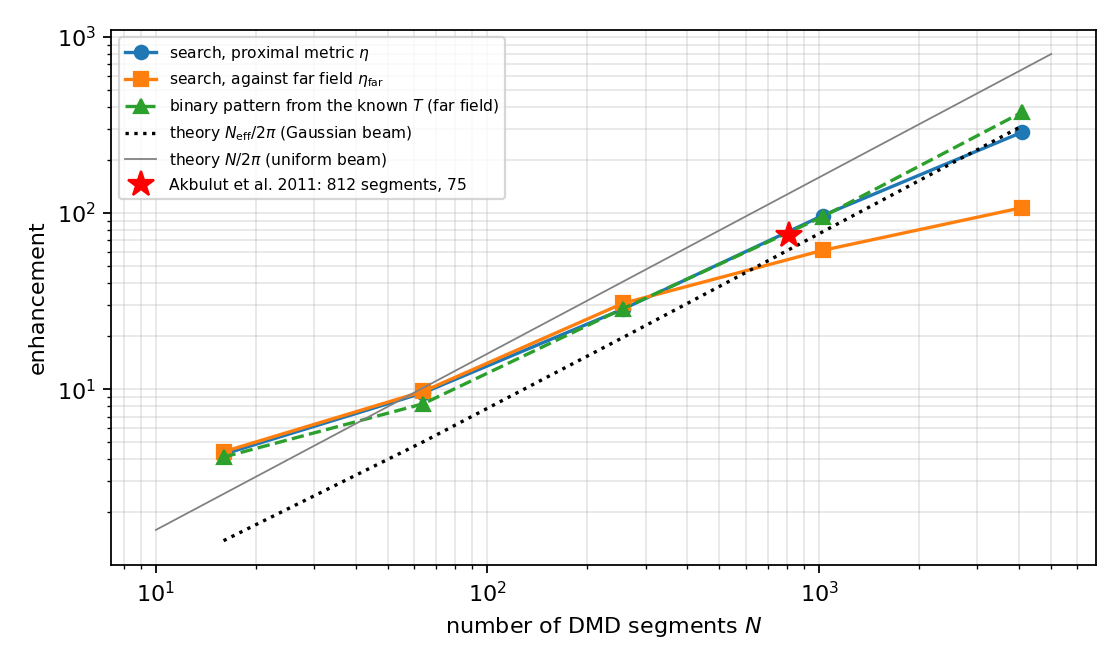
\includegraphics[width=0.62\linewidth]{../hw2_agentic_hardware/figures/validation_vs_N.png}
\caption{Enhancement against the number of segments on the simulated bench.}
\end{figure}

\paragraph{The proximal background can be gamed.} The ratio $\eta$ rises if the focus brightens \emph{or} the ring darkens, and
with many segments the search does both. With 256 segments:
\begin{center}\small\ringtable\end{center}
A narrow ring ($r=6$--$14$\,px) gives a proximal $\eta$ more than twice $\eta_\text{far}$; a wide ring keeps the two close. At
1024 and 4096 segments even the wide ring is partly darkened ($\eta=96.6$ vs $\eta_\text{far}=61.3$; $287$ vs $107$), and the
far-field value stays below the known-$T$ pattern, i.e.\ 20\,000 iterations do not converge there. A focus square larger than
the speckle grain lowers $\eta$ (averaging over a bright centre and darker edges). This is why the tool reports both numbers.

\newcommand{\agentsegments}{256}\newcommand{\agenteta}{47.0}\newcommand{\agentetafar}{20.2}\newcommand{\agentfarpct}{7.9}\newcommand{\agentring}{5--15}
\subsection*{The agent's run}
Request: \emph{Focus the beam.} --- nothing else was typed. Model: \texttt{claude-cli:claude-sonnet-5-5}.

\begin{longtable}{@{}r r r r c r r r c r r@{}}
\toprule exp & macropixel & segments & focus & ring $r$ [px] & regions & iterations & flips & remeasure & $\eta$ & $\eta_\text{far}$\\\midrule\endhead
1 & 8 & 64 & 3 & 5--15 & 8 & 20000 & 4$\to$1 & yes & 9.8$\pm$0.1 & 7.6\\
\rowcolor{yellow!25}2 & 4 & 256 & 3 & 5--15 & 8 & 40000 & 8$\to$1 & yes & 47.0$\pm$0.1 & 20.2\\
3 & 16 & 16 & 3 & 5--15 & 8 & 10000 & 2$\to$1 & yes & 2.7$\pm$0.1 & 2.6\\
\bottomrule
\end{longtable}
Kept by the agent: experiment 2, enhancement 47.0 (far field 20.2). Diagnostics only the simulation knows: noise-free 47.3, known-$T$ binary pattern 25.7 (far field), theory $N_\text{eff}/2\pi=19.6$.
\begin{figure}[H]\centering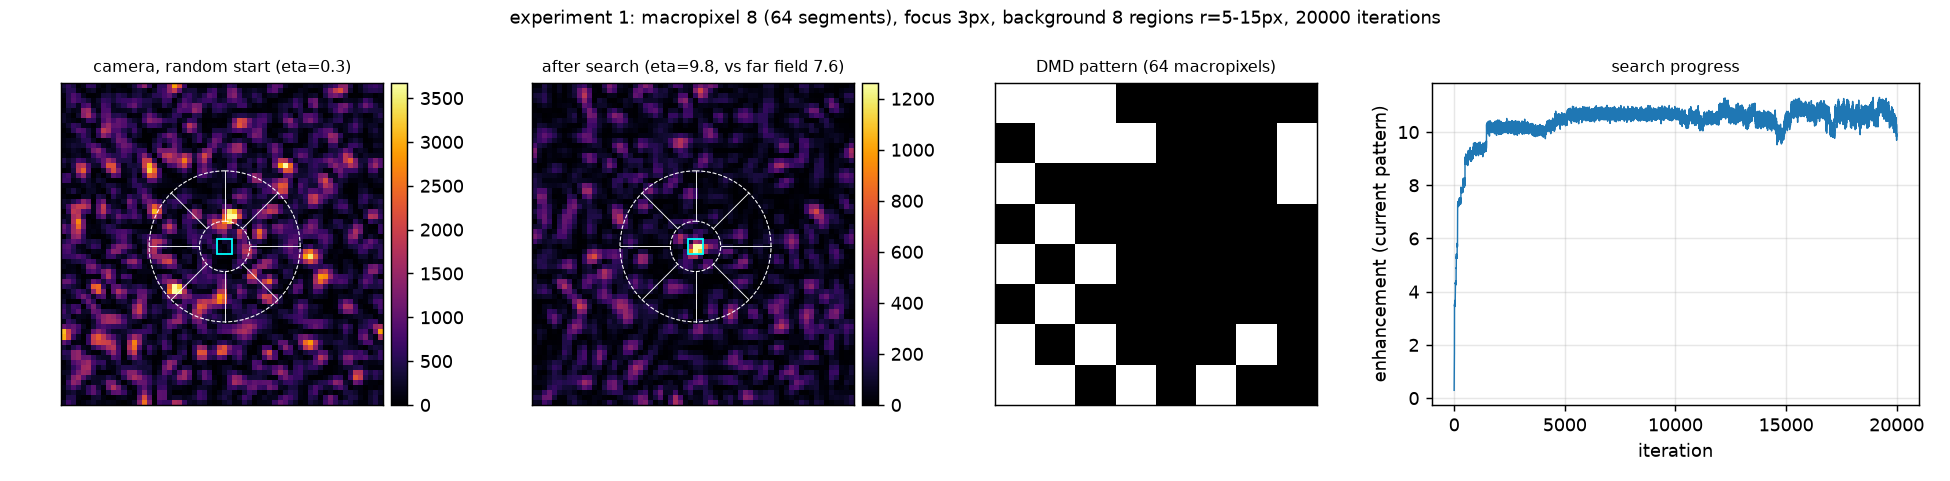
\includegraphics[width=\linewidth]{hw2_figs/agent_run/experiment_01.png}\caption{Agent experiment 1.}\end{figure}
\begin{figure}[H]\centering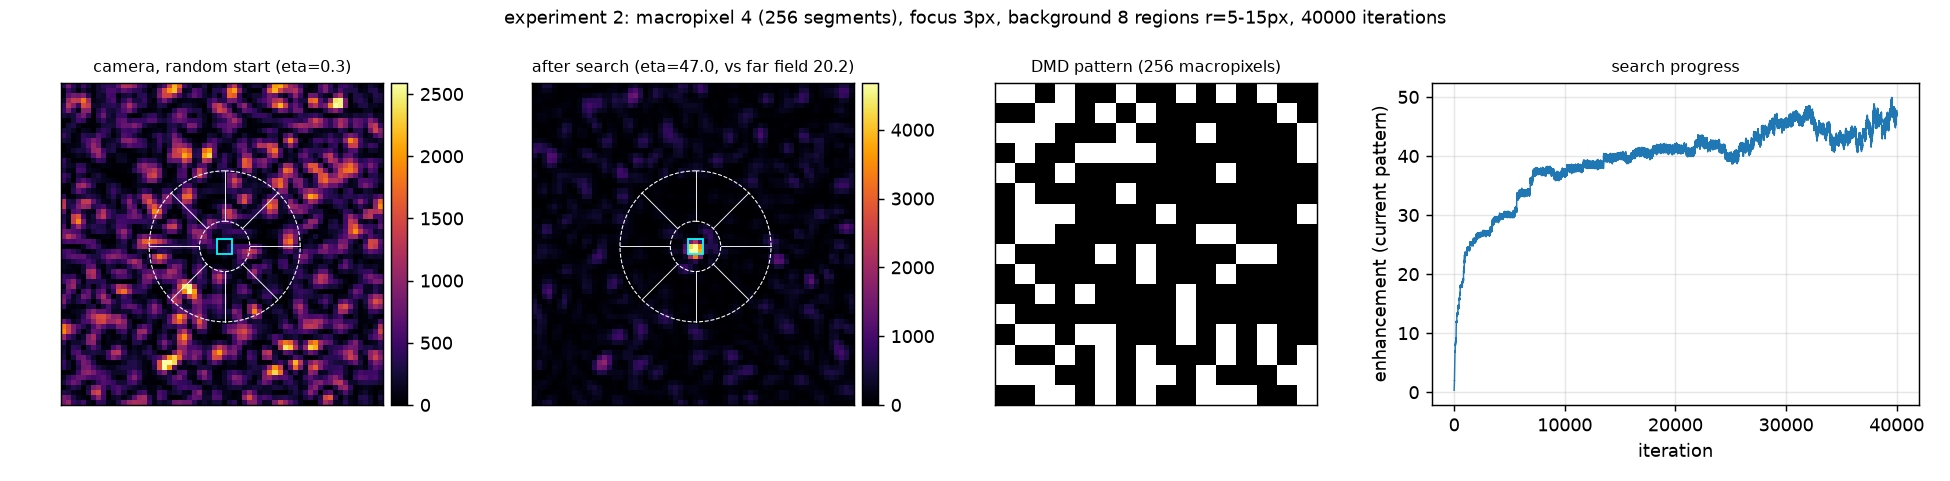
\includegraphics[width=\linewidth]{hw2_figs/agent_run/experiment_02.png}\caption{Agent experiment 2.}\end{figure}
\begin{figure}[H]\centering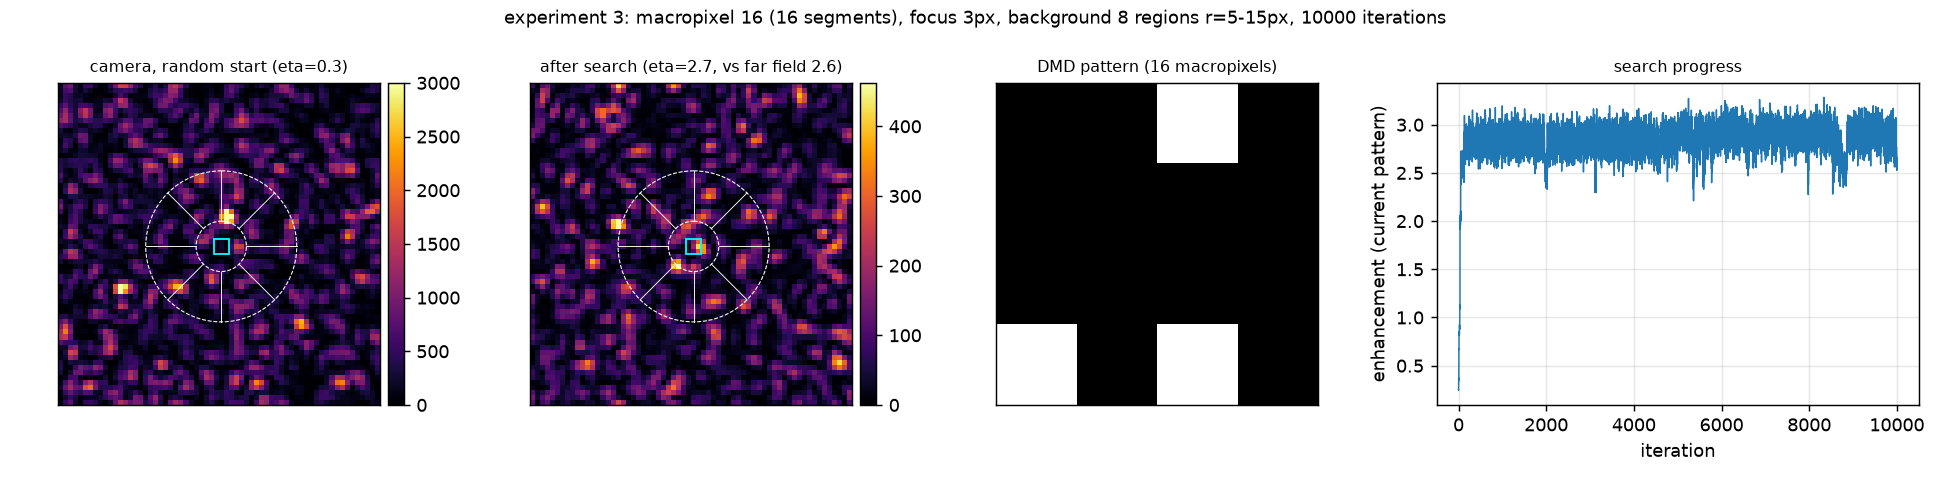
\includegraphics[width=\linewidth]{hw2_figs/agent_run/experiment_03.png}\caption{Agent experiment 3.}\end{figure}
\paragraph{Who did what.}
\begin{longtable}{@{}r l p{0.74\linewidth}@{}}
\toprule \# & role & what it did\\ \midrule \endhead
1 & user & Focus the beam.\\
2 & orchestrator & -\textgreater{} scientist: No plan exists yet, so the scientist must define the focusing procedure before the executor can run it.\\
3 & scientist & \# Plan: focus the beam with `focusing\_tool` The standing brief asks for an ODE and neural-network plan with a voltage RMSE test. The instruction in this turn is a beam...\\
4 & orchestrator & -\textgreater{} executor: A plan now exists and only the executor can run the tools to produce a verified measurement.\\
5 & executor & experiment 1: \{"macropixel": 8, "focus\_size": 3, "bg\_inner": 5, "bg\_outer": 15, "bg\_regions": 8, "iterations": 20000, "flips": 4, "flips\_final": 1, "remeasure": true, ...\\
6 & orchestrator & -\textgreater{} finish: A VERIFIED measurement exists and the budget is limited, so I'll report the results to the user.\\
\bottomrule
\end{longtable}


\subsection*{Comparison with the focusing result from the lecture}
\newcommand{\lecturebest}{33}
The best enhancement in the lecture's experiment was about $\lecturebest$. The focus the agent kept on the simulated bench
($\agentsegments$ segments) scores $\eta=\agenteta$ with the task's proximal-background metric, above the lecture's value, and
$\eta_\text{far}=\agentetafar$ against the rest of the camera, below it. The two numbers bracket the lecture's result because the
agent's narrow ring (\agentring\,px) let the search darken the background it is measured against (see the bench validation).
With a wide ring the same $\agentsegments$ segments give $\eta=28.5$ and $\eta_\text{far}=30.7$ (bench validation table),
close to the lecture's $\lecturebest$, and 1024 segments give $\eta_\text{far}=61.3$, almost twice it. So, on the measure that
cannot be raised by darkening the ring, the simulated bench with $\agentsegments$ segments is at the level of the lecture's
experiment and needs more segments to exceed it; a real bench also loses enhancement to drift and mechanical instability,
which the simulation does not have.

\paragraph{Published experiments and theory.}
For binary amplitude modulation the expected optimum is $\eta\approx N/2\pi$ (about $0.16N$), lower than phase-only shaping
($\eta\approx\pi N/4$) by a factor $\pi^2/2$. Akbulut et al.\ (Opt.\ Express 19, 4017, 2011) obtained $75\pm6$ with 812 segments
(theory $129$, i.e.\ $58\%$ of it); Zhang et al.\ report 152 with 1536 segments on a DMD with a genetic algorithm (9.9\% of $N$).
On the simulated bench the search reaches, against the far field, $9.7$ with 64 segments, $30.7$ with 256 and $61.3$ with 1024
(15\%, 12\% and 6.0\% of $N$; the Gaussian illumination gives $N_\text{eff}\approx N/2$), the same order as the experiments.
The focus the agent kept ($\agentsegments$ segments, ring \agentring\,px) has $\eta=\agenteta$ and
$\eta_\text{far}=\agentetafar$ (\agentfarpct\% of $N$): against the far field it is in the same range as the experiments,
while its proximal $\eta$ is more than twice $\eta_\text{far}$ because the agent chose a narrow ring, the effect shown in the
bench validation above.
Differences to keep in mind: the bench has no drift, no mechanical instability and a perfectly static medium, which favours the
simulation, while the noise and the finite iteration budget limit it at large $N$; and the task's proximal-background metric can
read higher than the usual definition (focus over the average speckle), as shown above.
\end{document}
